% Template for ICIP-2019 paper; to be used with:
%          spconf.sty  - ICASSP/ICIP LaTeX style file, and
%          IEEEbib.bst - IEEE bibliography style file.
% --------------------------------------------------------------------------
\documentclass{article}
\usepackage{spconf,amsmath,graphicx,lipsum,multicol}

% Example definitions.
% --------------------
\def\x{{\mathbf x}}
\def\L{{\cal L}}

% Title.
% ------
\title{A Method To Improve Accuracy of AMOLED Display Panel Quality Assessment By Using Contrast Sensitivity Function}
%
% Single address.
% ---------------
\name{Tong Liu\\
UW ID:20809932}
\address{University of Waterloo\\
        Department of Electrical and Computer Engineering\\
        200 University Ave W, Waterloo, Ontario, N2L 3G1, Canada}
%
% For example:
% ------------
%\address{School\\
%	Department\\
%	Address}
%
% Two addresses (uncomment and modify for two-address case).
% ----------------------------------------------------------
%
\begin{document}

\maketitle{}
%
\begin{abstract}
%
In this research project, author used the knowledge of Contrast Sensitivity Function which gained from previous review project, implemented Contrast sensitivity function code in both MATLAB and python code, applied to a python based AMOLED Display Panel quality assessment system. Author have done a numbers of tests and experiments by comparing different models of Contrast sensitivity function in the AMOLED display panel quality assessment system, finally selected one model based on the performance figures. By using this Contrast sensitivity function model to compare without using contrast sensitivity function, it clearly show there is big improvement of accuracy of the system to classify good and bad quality of AMOLED display Panels .   
\end{abstract}

\begin{keywords}
Contrast Sensitivity Function, Image Quality Assessment, Display Luminance Uniformity, AMOLED, AMOLED Display Ageing, Burn-in, MURA
\end{keywords}
%

\section{Introduction}
The AMOLED (Active Matrix Organic Light Emitting Diode) display panel has been used by high-end smart phone maker such as, Apple, Samsung, Google and so on, in their latest products. The market also shows a strong need of AMOLED display Panel in high end TV and Car displays industry. However, to adopt good quality AMOLED display panel into product, there are two issues which are impact AMOLED display performance. These issues all related to luminance performance of the AMOLED panel. First issue is luminance non-uniformity which is caused while AMOLED panel is manufactured in plant, as know as MURA - A Japanese term for "irregularity". The second is AMOLED display panel ageing issue, this is a long term performance issue, it is caused by OLED material ageing, which is the luminance performance drop at some heavily used area of panel, it lead to become another luminance non-uniformity issue, as know as image burn-in on AMOLED display. 
To address these issues an unique solution has been developed by author's engineering team, it's called non-uniformity and ageing compensation. See figure \ref{fig1}. \\

\begin{figure}[h]
\begin{minipage}[b]{.3\linewidth}
  \centering
  \centerline{
\includegraphics[width=1.8cm]{images/csfed_G_480_I0_PsdLum.png}}
%  \vspace{1.5cm}
  \centerline{(a) MURA}\medskip
\end{minipage}
\hfill
\begin{minipage}[b]{0.3\linewidth}
  \centering
  \centerline{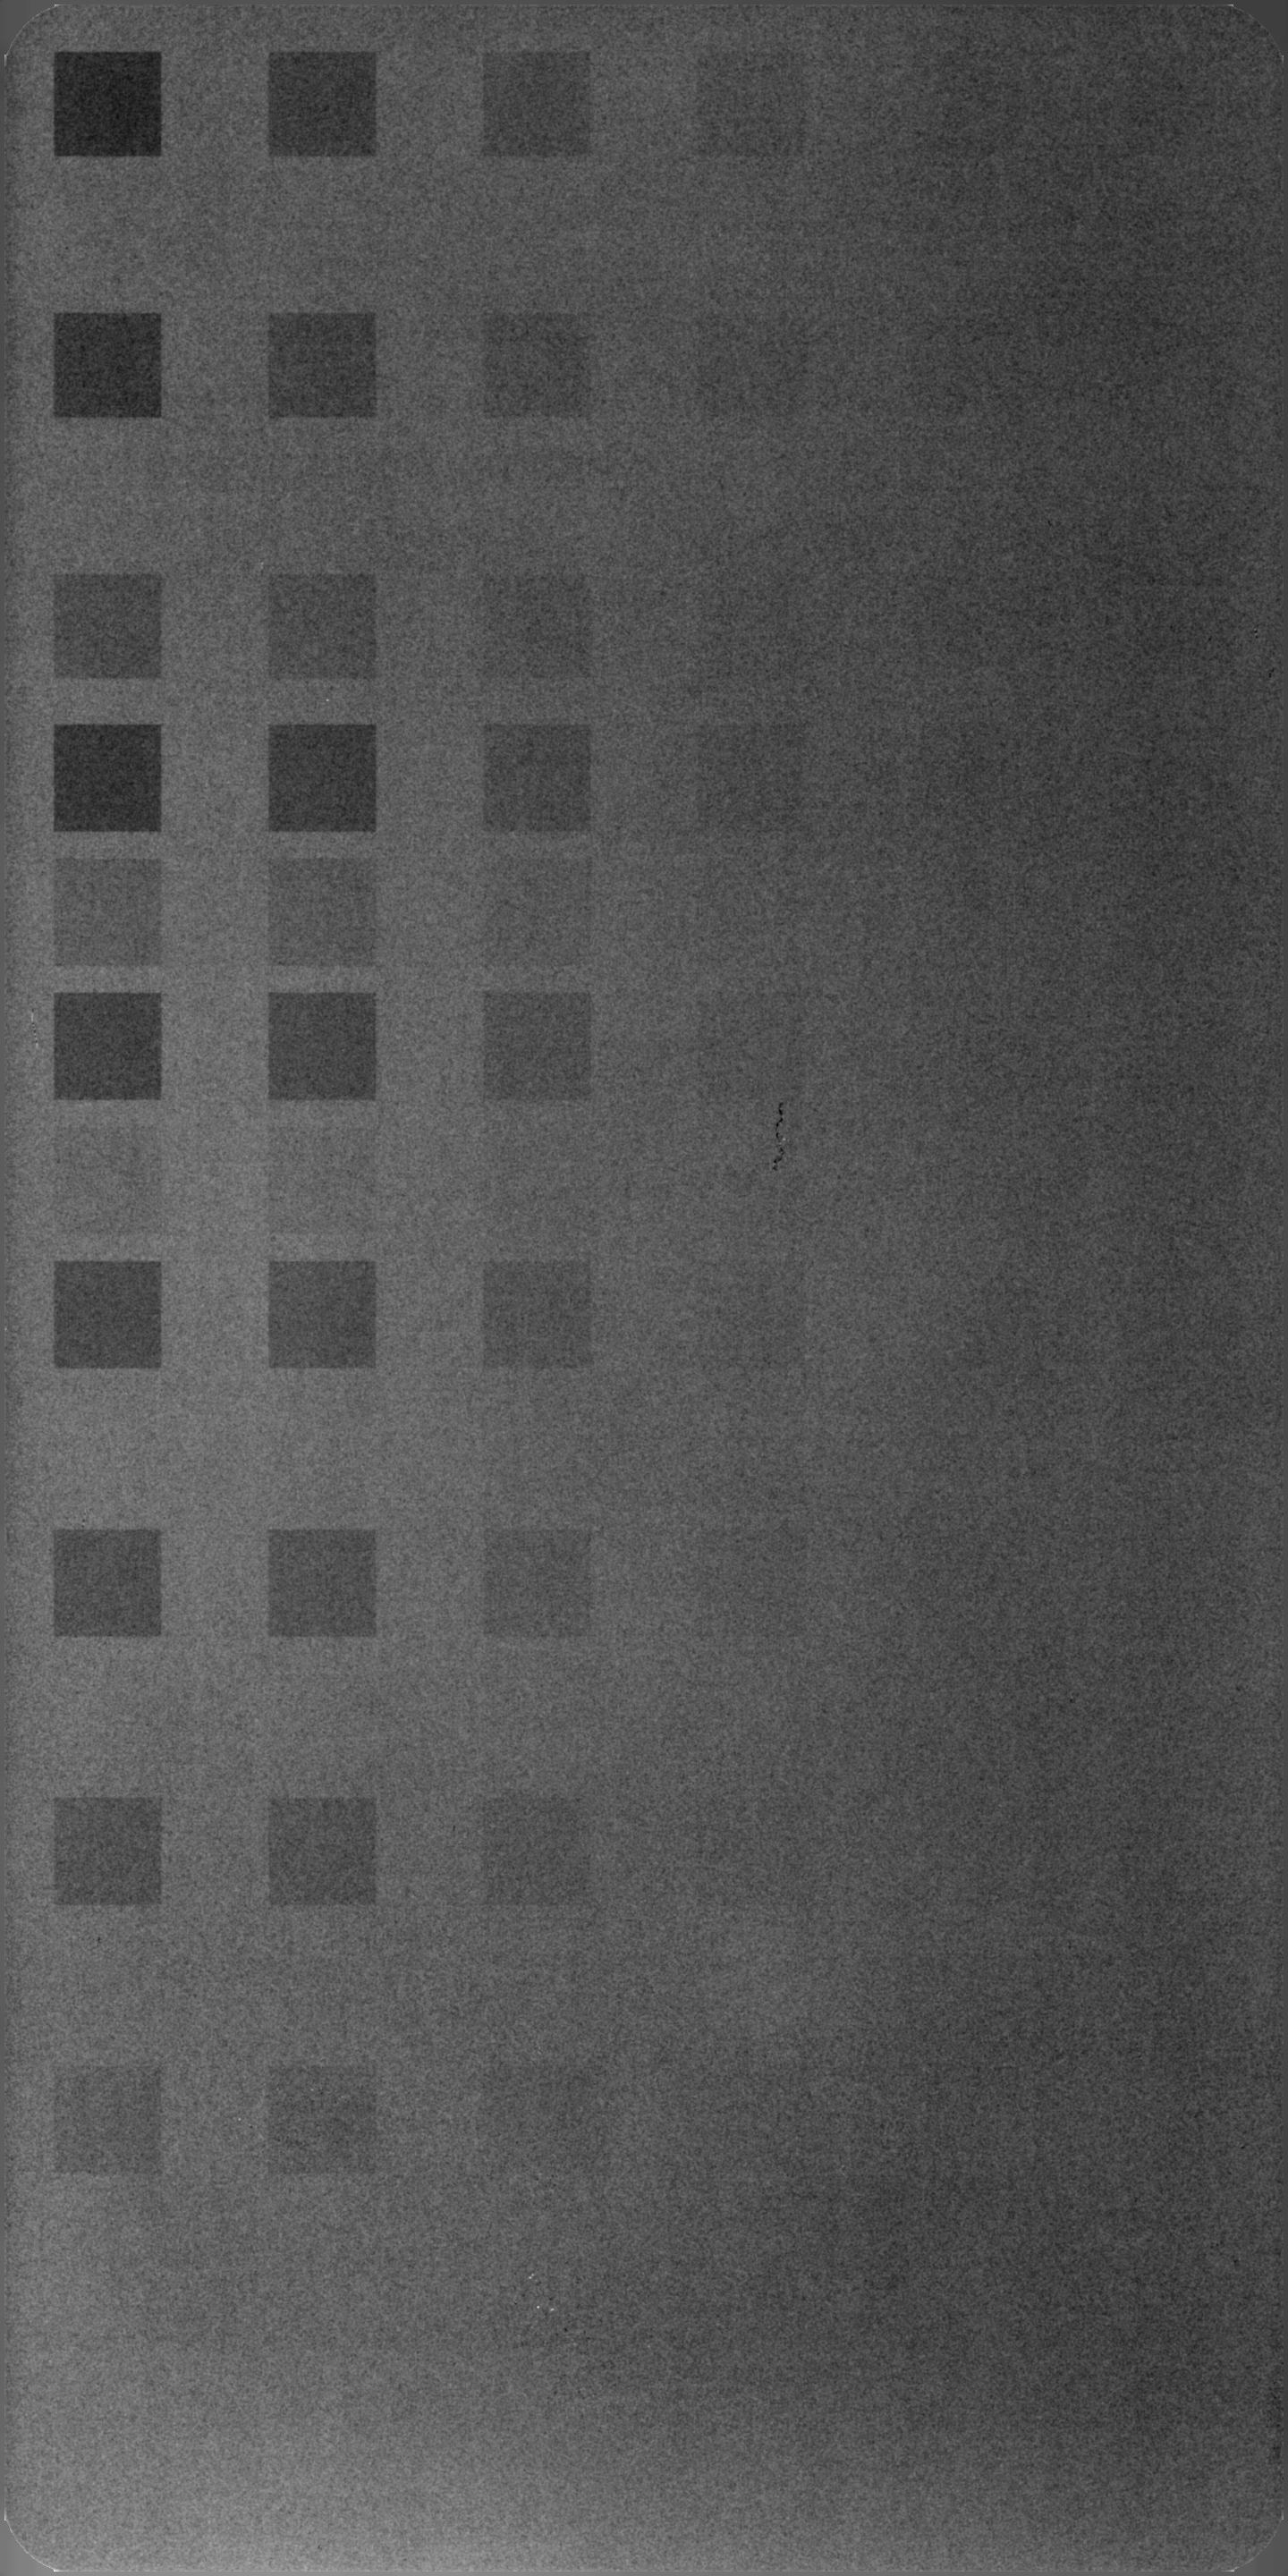
\includegraphics[width=1.8cm]{images/A1_G_300_I0_PsdLum.csv.png}}
%  \vspace{1.5cm}
  \centerline{(b) Burn-in }\medskip
\end{minipage}
%
\hfill
\begin{minipage}[b]{0.3\linewidth}
  \centering
  \centerline{
\includegraphics[width=1.8cm]{images/A1_G_300_I2_PsdLum.csv.png}}
%  \vspace{1.5cm}
  \centerline{(c) Compensated}\medskip
\end{minipage}
%
\caption{MURA, Burn-In and After Compensation}
\label{fig1}
%
\end{figure}
To evaluate the quality of compensation for both AMOLED panel's non-uniformity and ageing issues, author developed a rapid AMOLED display panel quality assessment system to evaluate the AMOLED panel compensation quality, which is checking luminance uniformity performance across AMOLED panel by analysing the compensated panel's gray-scale image via a CNN based auto-encoder. However without using any image pre-processing only takes original AMOLED panel gray-scale images as input, in the case of the luminance difference on AMOLED panel was small the system couldn't make clear decision of whether compensation was good or bad. 
In this research project author tried to address this issue by adopting contrast sensitivity function into the system as part of AMOLED panel image pre-processing to improve the overall performance of the system. \\

\section{AMOLED display Quality Assessment System And Its Improvement }
The figure \ref{fig_sys_diagram} shows the AMOLED display panel quality assessment system architecture. 
\subsection{Pre-processing}
The pre-processing block originally only does image data cleansing and resizing, then output to auto-encoder as its input. In this research project author added contrast sensitivity function filter as additional part of image pre-processing. According to the previous review project study, the contrast sensitivity function can help to remove human visual system's subjective effect, then Contrast Sensitivity Function filtered image can emphasis the small luminance error across AMOLED panel, therefore increase the AMOLED panel quality assessment accuracy. 
\subsection{Auto-encoder}
In order to compare the AMOLED display panel original image and the reference image to judge the panel compensation quality. Use original image as test image which may contains not fully eliminated MURA or Burn-in image error. Author modified a CNN (Convolutional Neural Network) based auto-encoder python program which originally developed by Alyssa Huang and author \cite{657A_report}. Auto-encoder was used  to create the reference image of panel by using original panel image as input, the auto-encoder eliminates original image's error which caused by MURA ,burn-in or low quality compensation.  
\subsection{Evaluation process}
This part is evaluation process. This process includes two steps. First step is post auto-encoder processor, it computes two performance indicator factors Cosine similarity and Mean square error. The second step use those two performance indicators as input ,runs a KNN classifier to classify the panel's quality is good or bad.
\begin{figure}[h]
    \centering
    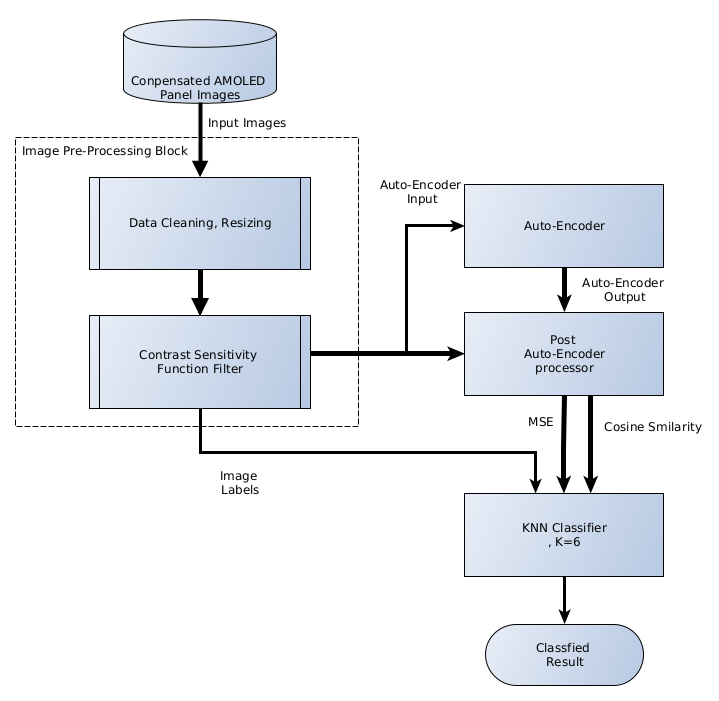
\includegraphics[width=0.52\textwidth]{images/system_diagram.png}\vfill
    \caption{AMOLED Panel Quality Assessment System Diagram}
    \label{fig_sys_diagram}
\end{figure}
\section{Apply Contrast Sensitivity Function Into System}
Based on the study in previous review project, author design and implemented process to apply contrast sensitivity function into the AMOLED display panel quality assessment system. Below discuss the details of process as high level requirement for actual code development.
\subsection{Coordinate Transformation}
Based on input image $I(x,y)$, where (x,y) is pixel location, then after FFT get spatial frequency domain image $\Theta(u,v)$, where, $u,v$ are spatial frequency on x, and y axis. before apply Contrast Sensitivity Function, we need to transform coordinate from x,y axis to polar coordinate by using following formula.
\begin{equation}
    \centering
    \label{eq:coor}
     r = \sqrt{u^2+v^2}
\end{equation}

\subsection{Apply FFT to image}
Apply Fast Fourier Transform filter to cleaned and resized original image by using fft2() and fftshift() functions in MATLAB.

\subsection{Apply Contrast Sensitivity Function}
Original Image is given as $I(x,y)$, fast Fourier transformed image is $\Phi(u,v)$, the contrast sensitivity function is $\Theta(r)$, then by multiplying two components $\Phi$ and $\Theta$, we get contrast sensitivity function filtered image $\hat{\Phi}(u,v)$.
\begin{equation}
    \centering
    \label{eq:applyCSF}
    \hat{\Phi}(u,v) = \Phi(u,v)\Theta(r) 
\end{equation}
\subsection{Apply inverse Fast Fourier Transform}
Apply inverse Fast Fourier Transform filter to CSF filtered image $\hat{\Phi}(u,v)$ by using ifft2() and ifftshift() functions in MATLAB.

\section{Apply Different Contrast Sensitivity Function models}
There are many different CSF models were published by different researchers. In this research from simplicity of implementation prospective, author picked four different models for comparison, at end chose one model which has the best performance.\\
Equations of these models are listed as below.
\subsection{Daly model, 1993\cite{UseCSFinFusedIMage}}
\begin{equation}
    \centering
    \label{eq:daly}
     \Theta(r) = (\frac{0.008}{r^3}+1)^{-0.2}1.42re^{-0.3u\sqrt{1+0.06e^{0.3r}}}
\end{equation}
\subsection{DoG model, Watsonand Ahumada 2005\cite{Standard-Model-Contrast}}
\begin{equation}
    \centering
    \label{eq:DoG}
     \Theta(r) = e^{-(r/r_0)^2}-ae^{-(r/r_1)^2}
\end{equation}
Where, $r_0 = 15.3870$, $r_1 = 1.3456$, $a = 0.7622$.
\subsection{Barton model, \cite{AssessmentAlgoImageFusion}}
\begin{equation}
    \centering
    \label{eq:mannos}
     \Theta(r) = re^{-0.25r}
\end{equation}
Where a = 75, b =0.2, and c = 0.8. 
\subsection{Mannos And Sakrison model,\cite{Mannos-Sakrison}}
\begin{equation}
    \centering
    \label{eq:mannos}
     \Theta(r) = 2.6(0.0192+0.144r)e^{-(0.144r)^{1.1}}
\end{equation}

\section{Experiments}
In order to verify how much the contrast sensitivity function will help for classify the quality of compensation for AMOLED display panels. Author used two sets of image data, one set is known has good compensation quality those images were labeled as "comp". Another set of data is known hasn't good compensation quality or not have compensated at all, these images were labeled as "uncomp". There are two goals for the experiment.\\
First goal is at end of process to check whether the system can classify these two sets of data based on those two quality indicators - Cosine similarity and MSE. Based on the contrast sensitivity function theory, Author expected the experiment result of using CSF filtered image will better than the result of without using CSF filtered image.\\
Second goal is in case of using Contrast sensitivity function, iterate through different CSF models, depends on the result to choose the best performed CSF model.
\subsection{Experiment Procedure}
Experiments were follow below procedure. It is separated to two phases.\\
First, pre-process images with contrast sensitivity function filter,and iterated with different Contrast sensitivity function model in each iteration. This part is done with MATLAB code.
\begin{itemize}
    \item put pre-classified images into "comp" and "uncomp" two folders, 
    \item Load AMOLED display panel image which acquired by separated optical measurement system
    \item Apply a Contrast stretch Transformation for the input image in matlab
    \item Apply Contrast Sensitivity Function to the image in matlab
    \item Output the CSF filtered image stored as new image file in matlab
\end{itemize}
The second, this part loads CSF filtered images and original images run through auto-encoder and perform evaluation calculation, this part is done by python code.
\begin{itemize}
    \item Load image from "comp" and "uncomp" folders, create data matrices with flattened input image data as samples. Label each sample as "comp" or "uncomp" based on which folder the image was loaded from.
    \item run auto-encoder with image matrices as input, save the output
    \item run evaluation process use auto-encoder input and output image matrices as parameter, get Cosine Similarity and MSE, plot Cosine similarity and MSE, use cosine similarity as Y axis, and MSE as X axis. In the plot, the data point corresponds to "comp" image shown in blue color, in contrast, "uncomp" image data points shown in red color.   
\end{itemize}

\section{Experiment Results and Discussion}
\subsection{Non-CSF filtered vs CSF filtered}
\subsubsection{Difference Impacts In Pre-process phase}
Author chose DoG model to represent the case of using Contrast sensitivity Function to compare to the case of without using any contrast sensitivity function to pre-process the image.  
The figure \ref{fig3} shows the contrast between  original after compensation AMOLED display panel quality image and its CSF filtered image. The original image was taken at the luminance level on one smart phone AMOELD panel. the luminnance level is $300 cd/m^2$. As we can see it is almost invisible of any luminance non-uniformity error in the original images. However, from its CSF filtered images it is easy to detect the luminance non-uniformity spots in highlighted areas of the image. This is one indicator shows that the contrast sensitivity function can help to improve image quality judgement by removing the subjective effect of human eyes. The luminance non-uniformity error was emphasised by contrast sensitivity function filtering.

\begin{figure}[h]
\begin{minipage}[b]{.48\linewidth}
  \centering
  \centerline{
\includegraphics[width=2cm]{images/A1_G_300_I3_PsdLum.csv.png}}
%  \vspace{1.5cm}
  \centerline{(a) No CSF Filtered}\medskip
\end{minipage}
\hfill
\begin{minipage}[b]{0.48\linewidth}
  \centering
  \centerline{
\includegraphics[width=2cm]{images/DoG_csfed_A1_G_300_I3_PsdLum.csv.png}}
%  \vspace{1.5cm}
  \centerline{(b) CSF DoG Model Filtered}\medskip
\end{minipage}
%
\caption{Difference of Images Without and With Apply CSF Filter}
\label{fig3}
%
\end{figure}

\subsubsection{Difference Impacts In Final Result}
After verifying the improvement of applying contrast sensitivity function in pre-processing phase, let's take a look at how much of this improvement impacted the final result. Figure \ref{fig4} shows the result of after run through auto-encoder, how quality indicators of each image was distributed in comparison of with and without contrast sensitivity function filtering.  On the left side of figure\ref{fig4}-a, it shows that without applying contrast sensitivity function, the result of compensated AMOLED display panel image were distributed in a wider area. The blue data point which indicates to compensated panel images, and red data point which indicates to badly or no compensated panel images, these two type of images were clearly spreaded in the all area. In contrast, on the right side of figure \ref{fig4}-b, it shows that with contrast sensitivity function applied, the result of compensated AMOLED display panel image were concentrated in smaller area, and the blue color data points and read color data points were clearly separated, ans stay in their own region. This shows strong evidence of the contrast sensitivity function helps the system to classify the AMOLED display panel compensation quality, which lead to higher accuracy result of compensation quality assessment system.   

\begin{figure}[h]
\begin{minipage}[b]{0.48\linewidth}
  \centering
  \centerline{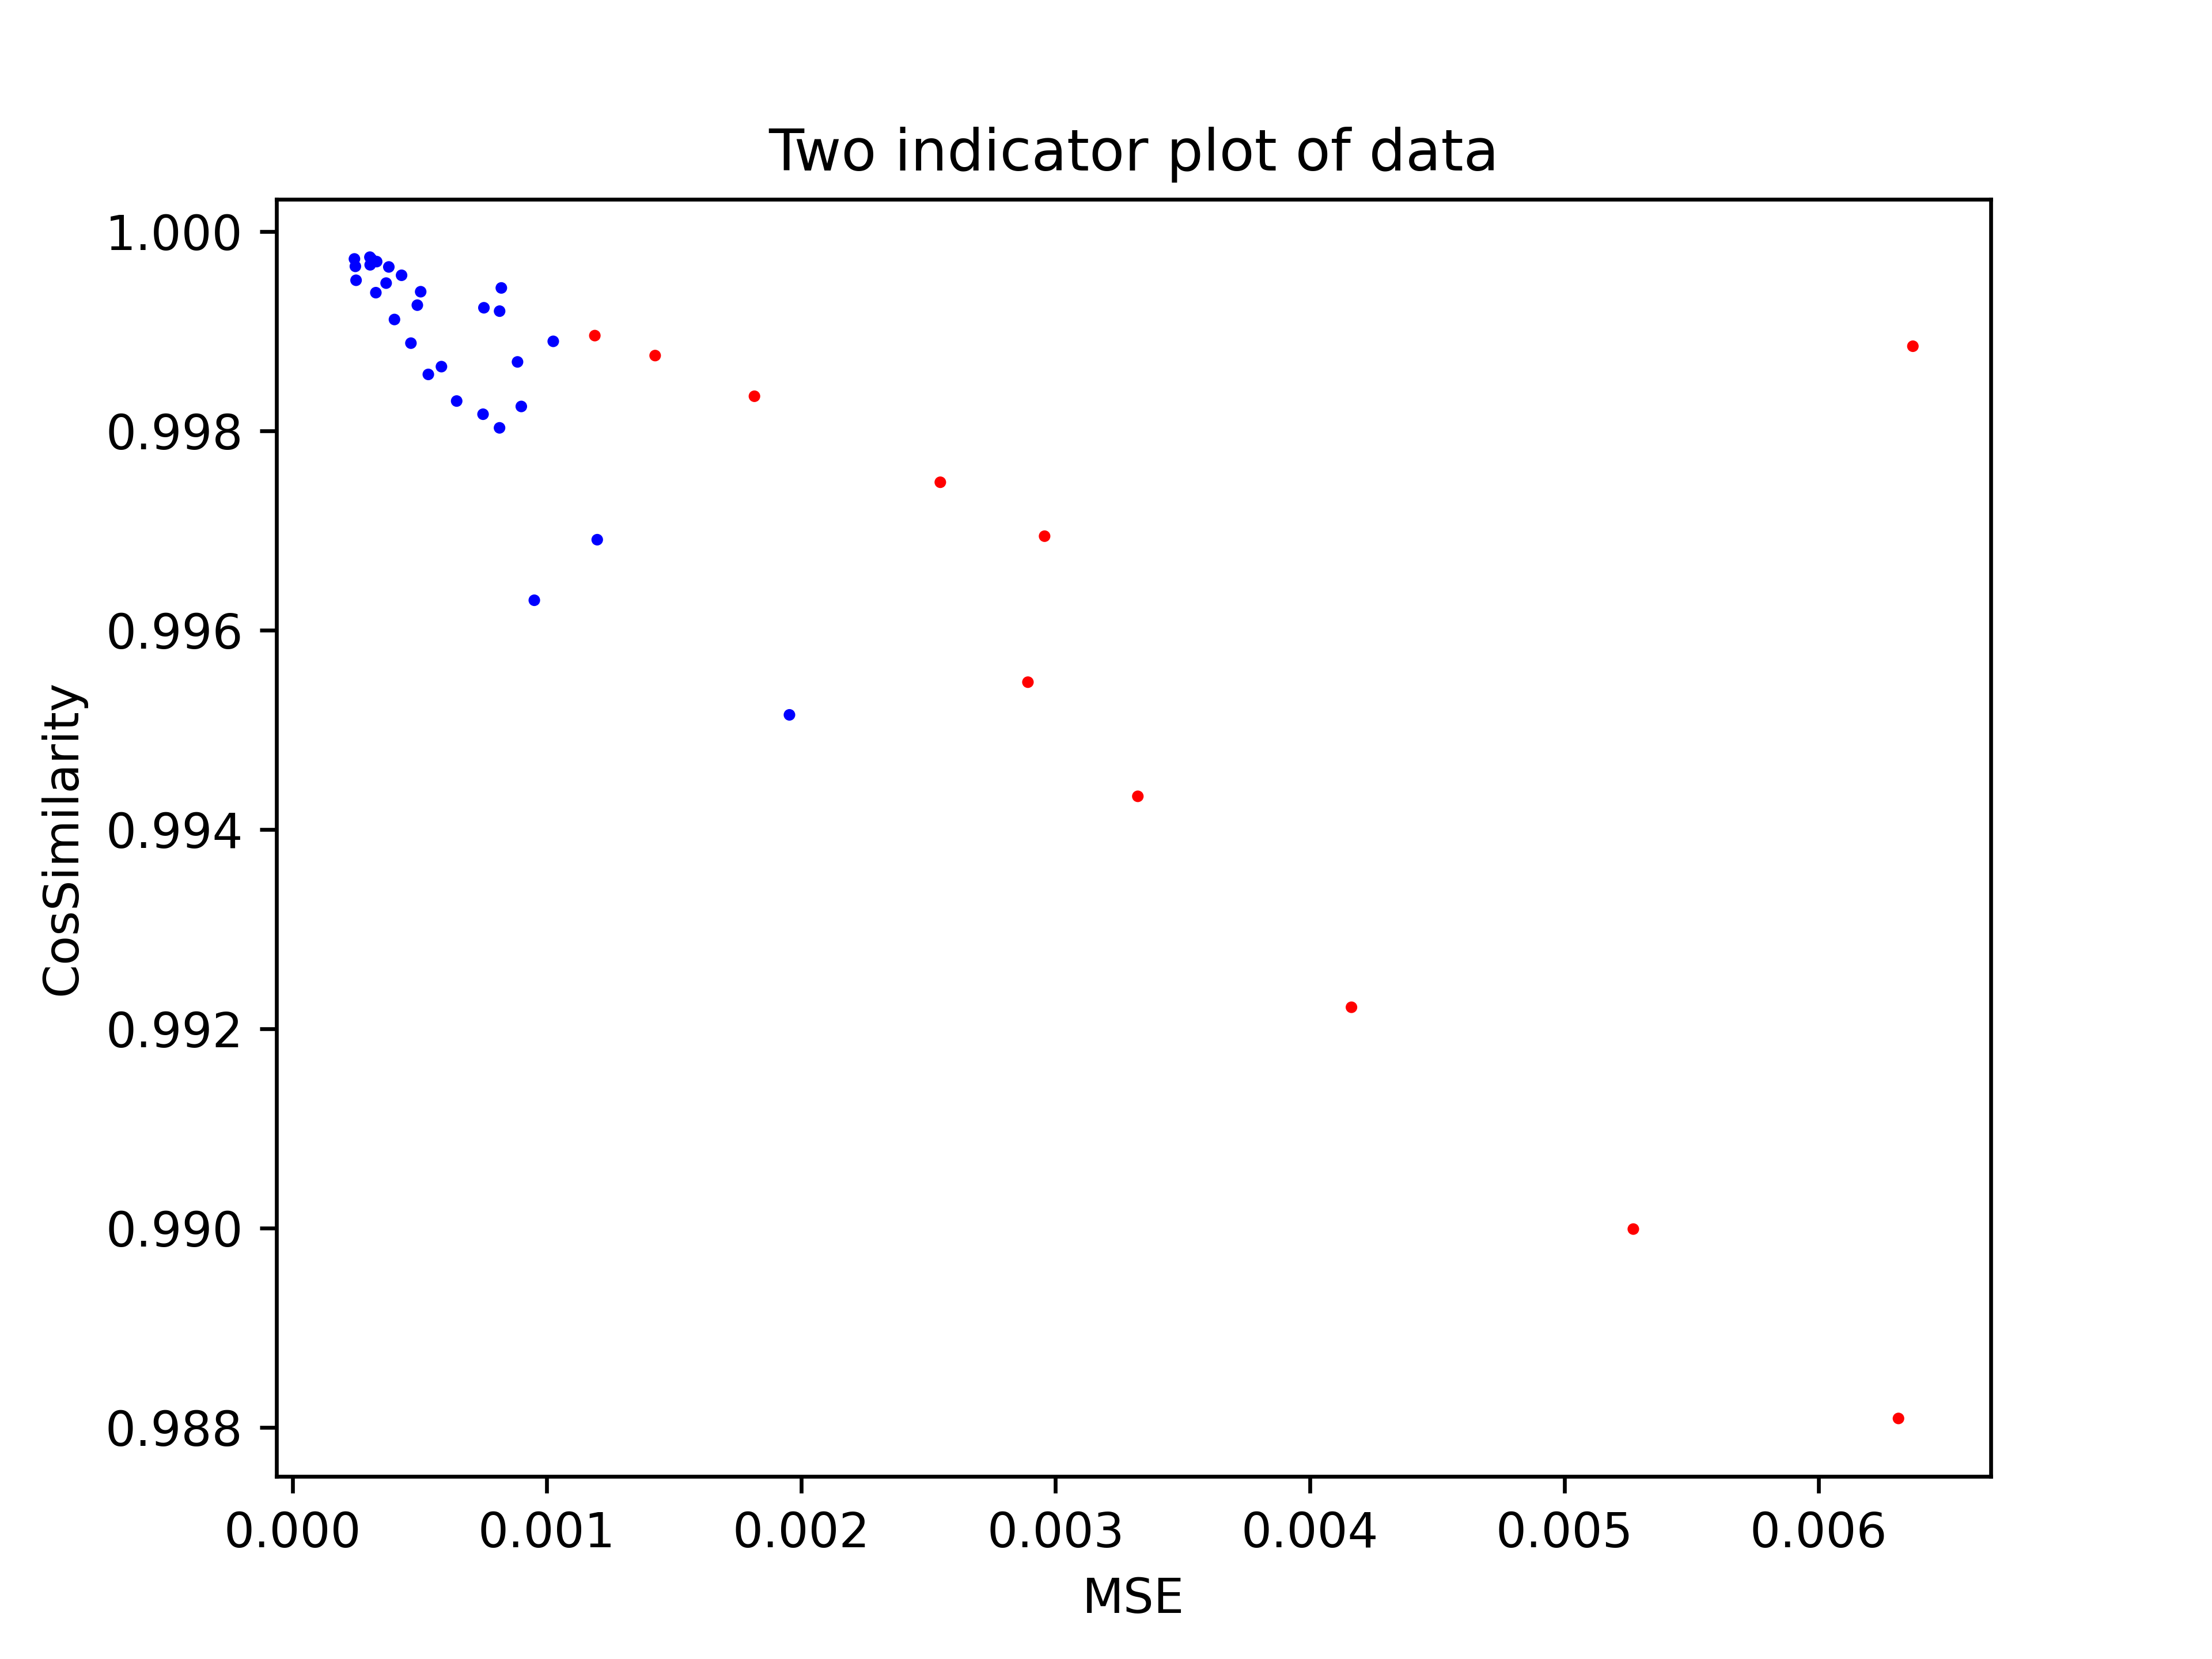
\includegraphics[width=4.0cm]{images/1440P_NoCSFed_0r_123b_result.png}}
%  \vspace{2.0cm}
  \centerline{(a) No CSF Filtered}\medskip
\end{minipage}
\hfill
\begin{minipage}[b]{0.48\linewidth}
  \centering
  \centerline{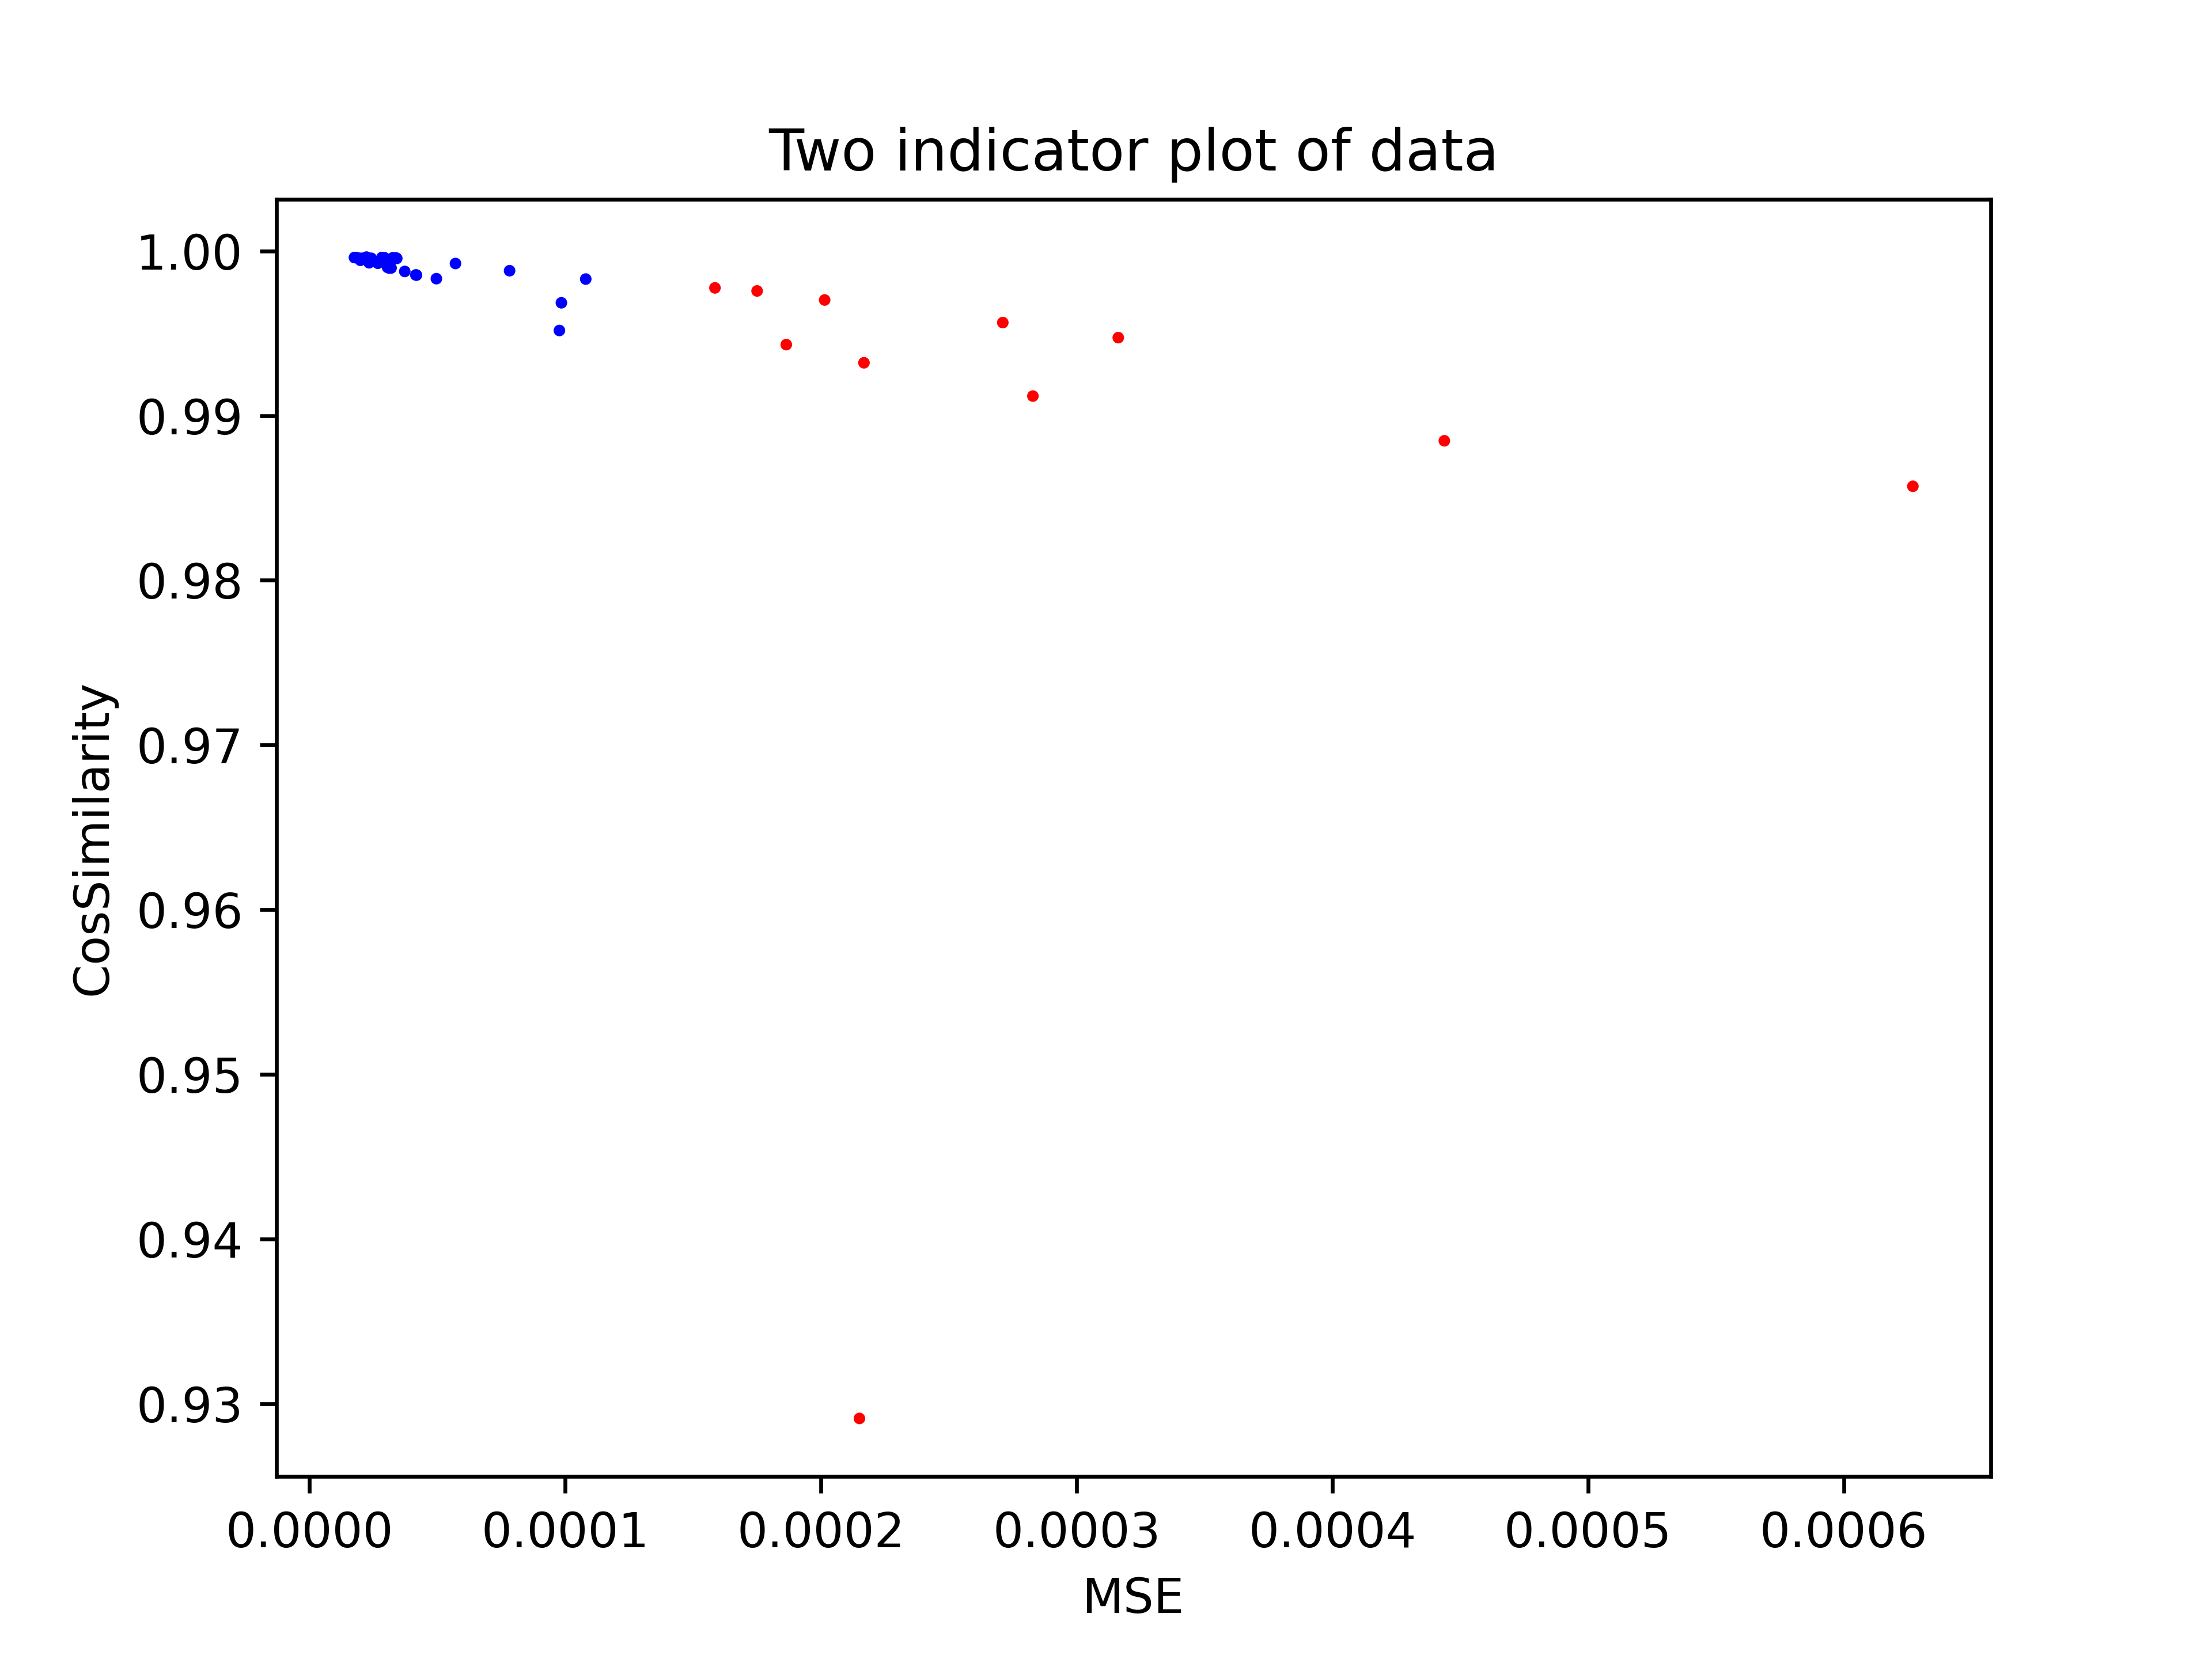
\includegraphics[width=4.0cm]{images/1440P_CSFed_0r_123b_result.png}}
%  \vspace{2.0cm}
  \centerline{(b)  CSF(DoG) Filtered}\medskip
\end{minipage}
%
\caption{Result of Without and with Apply CSF filter}
\label{fig4}
%
\end{figure}
\subsection{Comparison Between Different CSF models}

Above section discussed the experiments result which archived first goal of this project, which is prove the contrast sensitivity function does help to improve the the system assessment quality. For the second goal of this project author ran a big number of iteration of the experiment to find out which model has the best performance in terms of improve assessment quality of the compensation of AMOLED display panel. Figure \ref{fig5} shows plots of final result of different contrast sensitivity function model. These results were based on same group of sample images of AMOLED display panels, those images were grouped to be "comp" and "uncomp" two datasets. "comp" images are well compensated panel images, and blue dots indicate "comp" images. In contrast "uncomp" images are bad compensated or non-compensated images, and red dots indicate "uncomp" images.

\begin{figure}[h]
\begin{minipage}[b]{0.48\linewidth}
  \centering
  \centerline{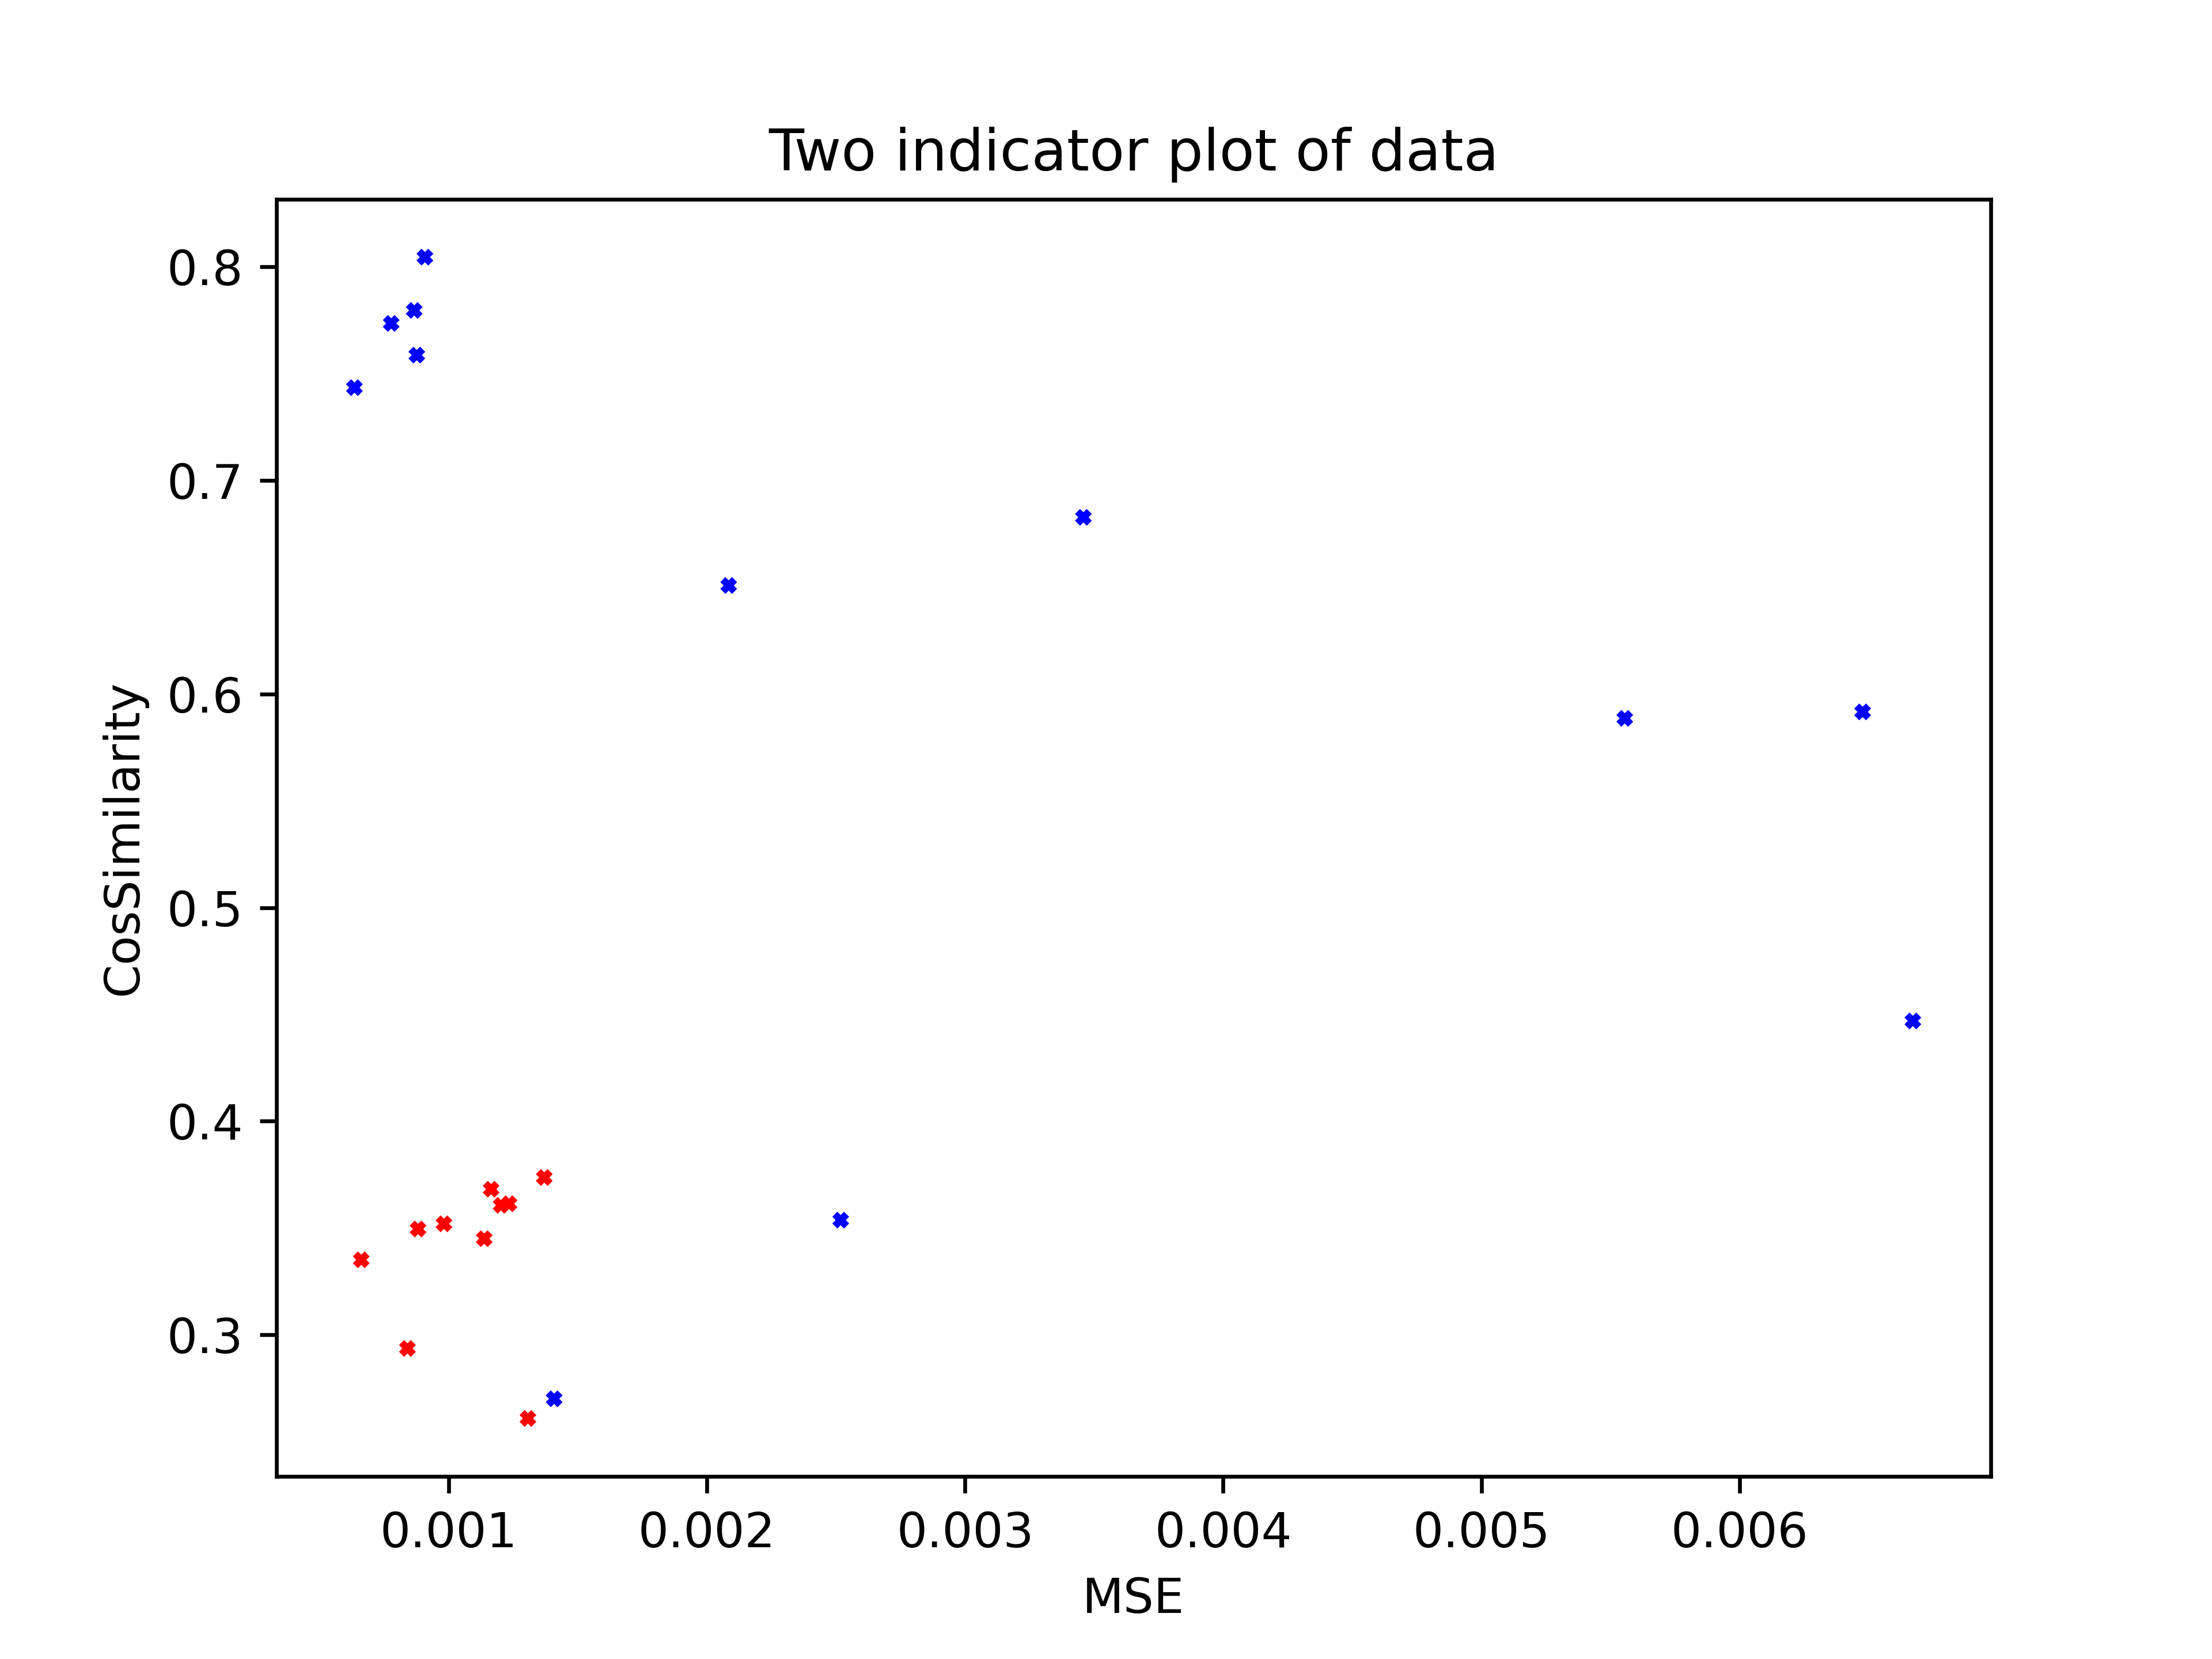
\includegraphics[width=4.0cm]{images/Barton_CSFed_G_A4_01R_23b_result.png}}
%  \vspace{2.0cm}
  \centerline{(a) Barton Model}\medskip
\end{minipage}
\hfill
\begin{minipage}[b]{0.48\linewidth}
  \centering
  \centerline{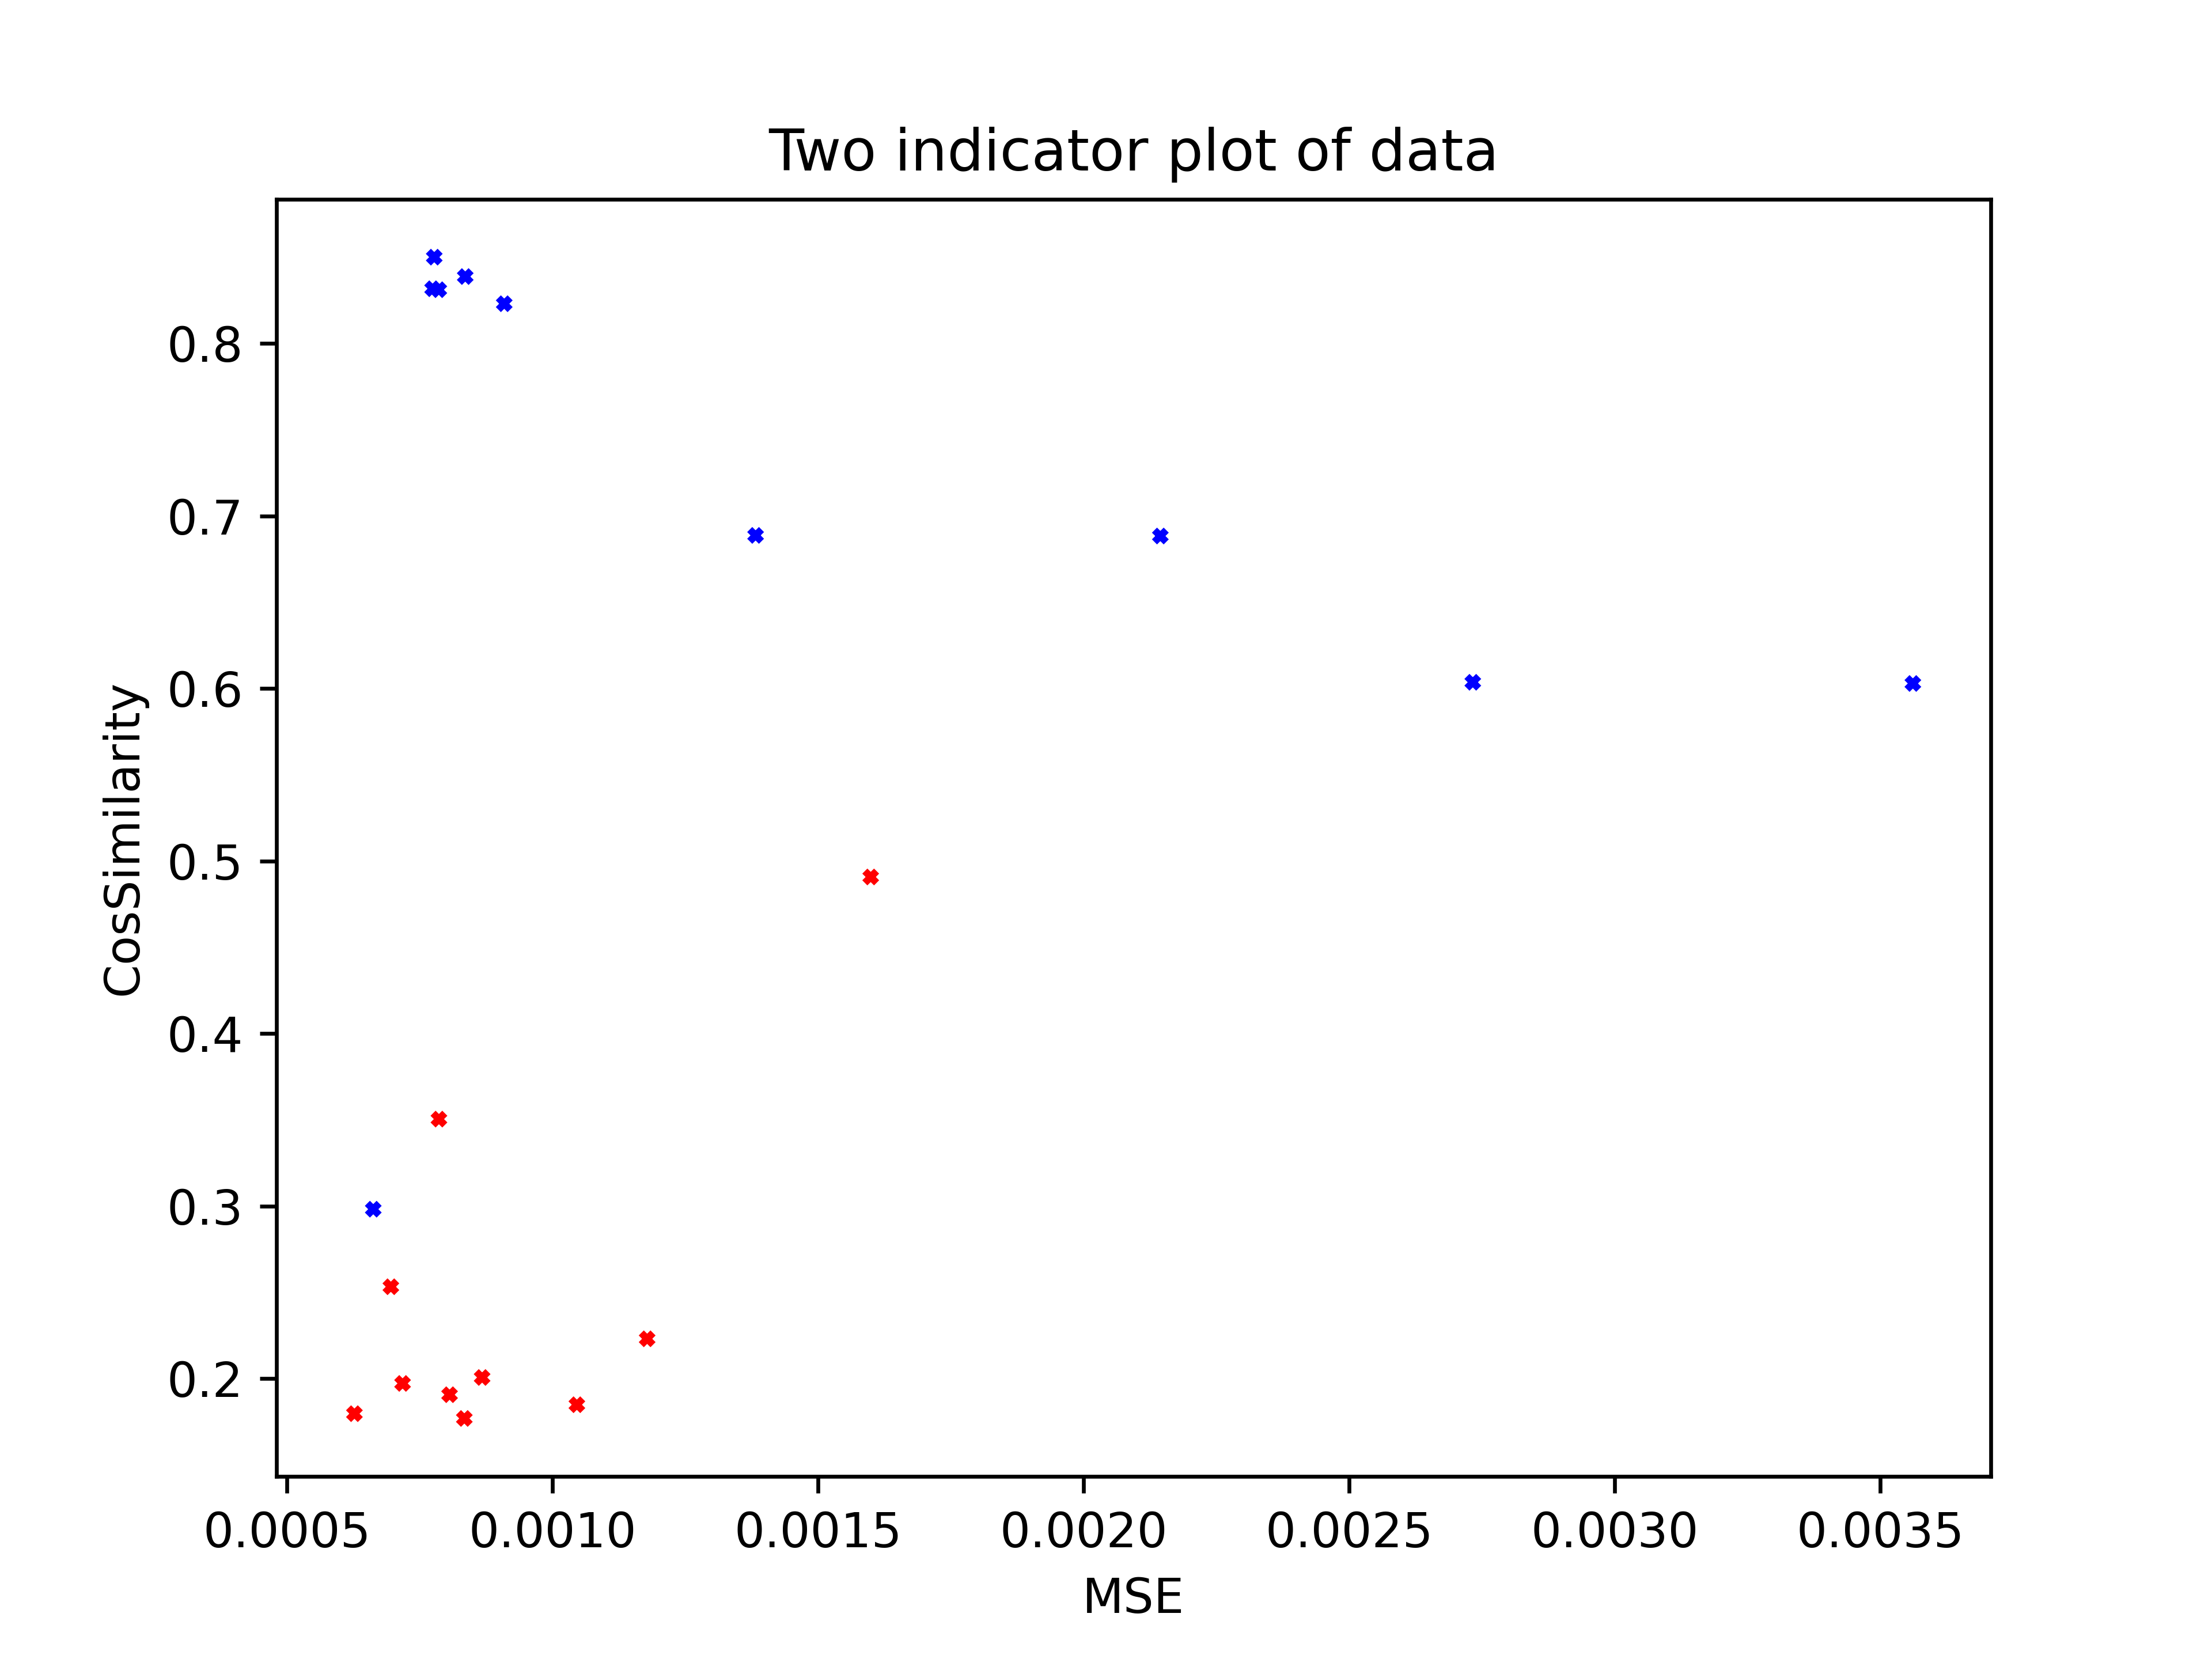
\includegraphics[width=4.0cm]{images/Daly_CSFed_G_A4_01r_23b_result.png}}
%  \vspace{2.0cm}
  \centerline{(b)  Daly Model}\medskip
\end{minipage}
\begin{minipage}[b]{.48\linewidth}
  \centering
  \centerline{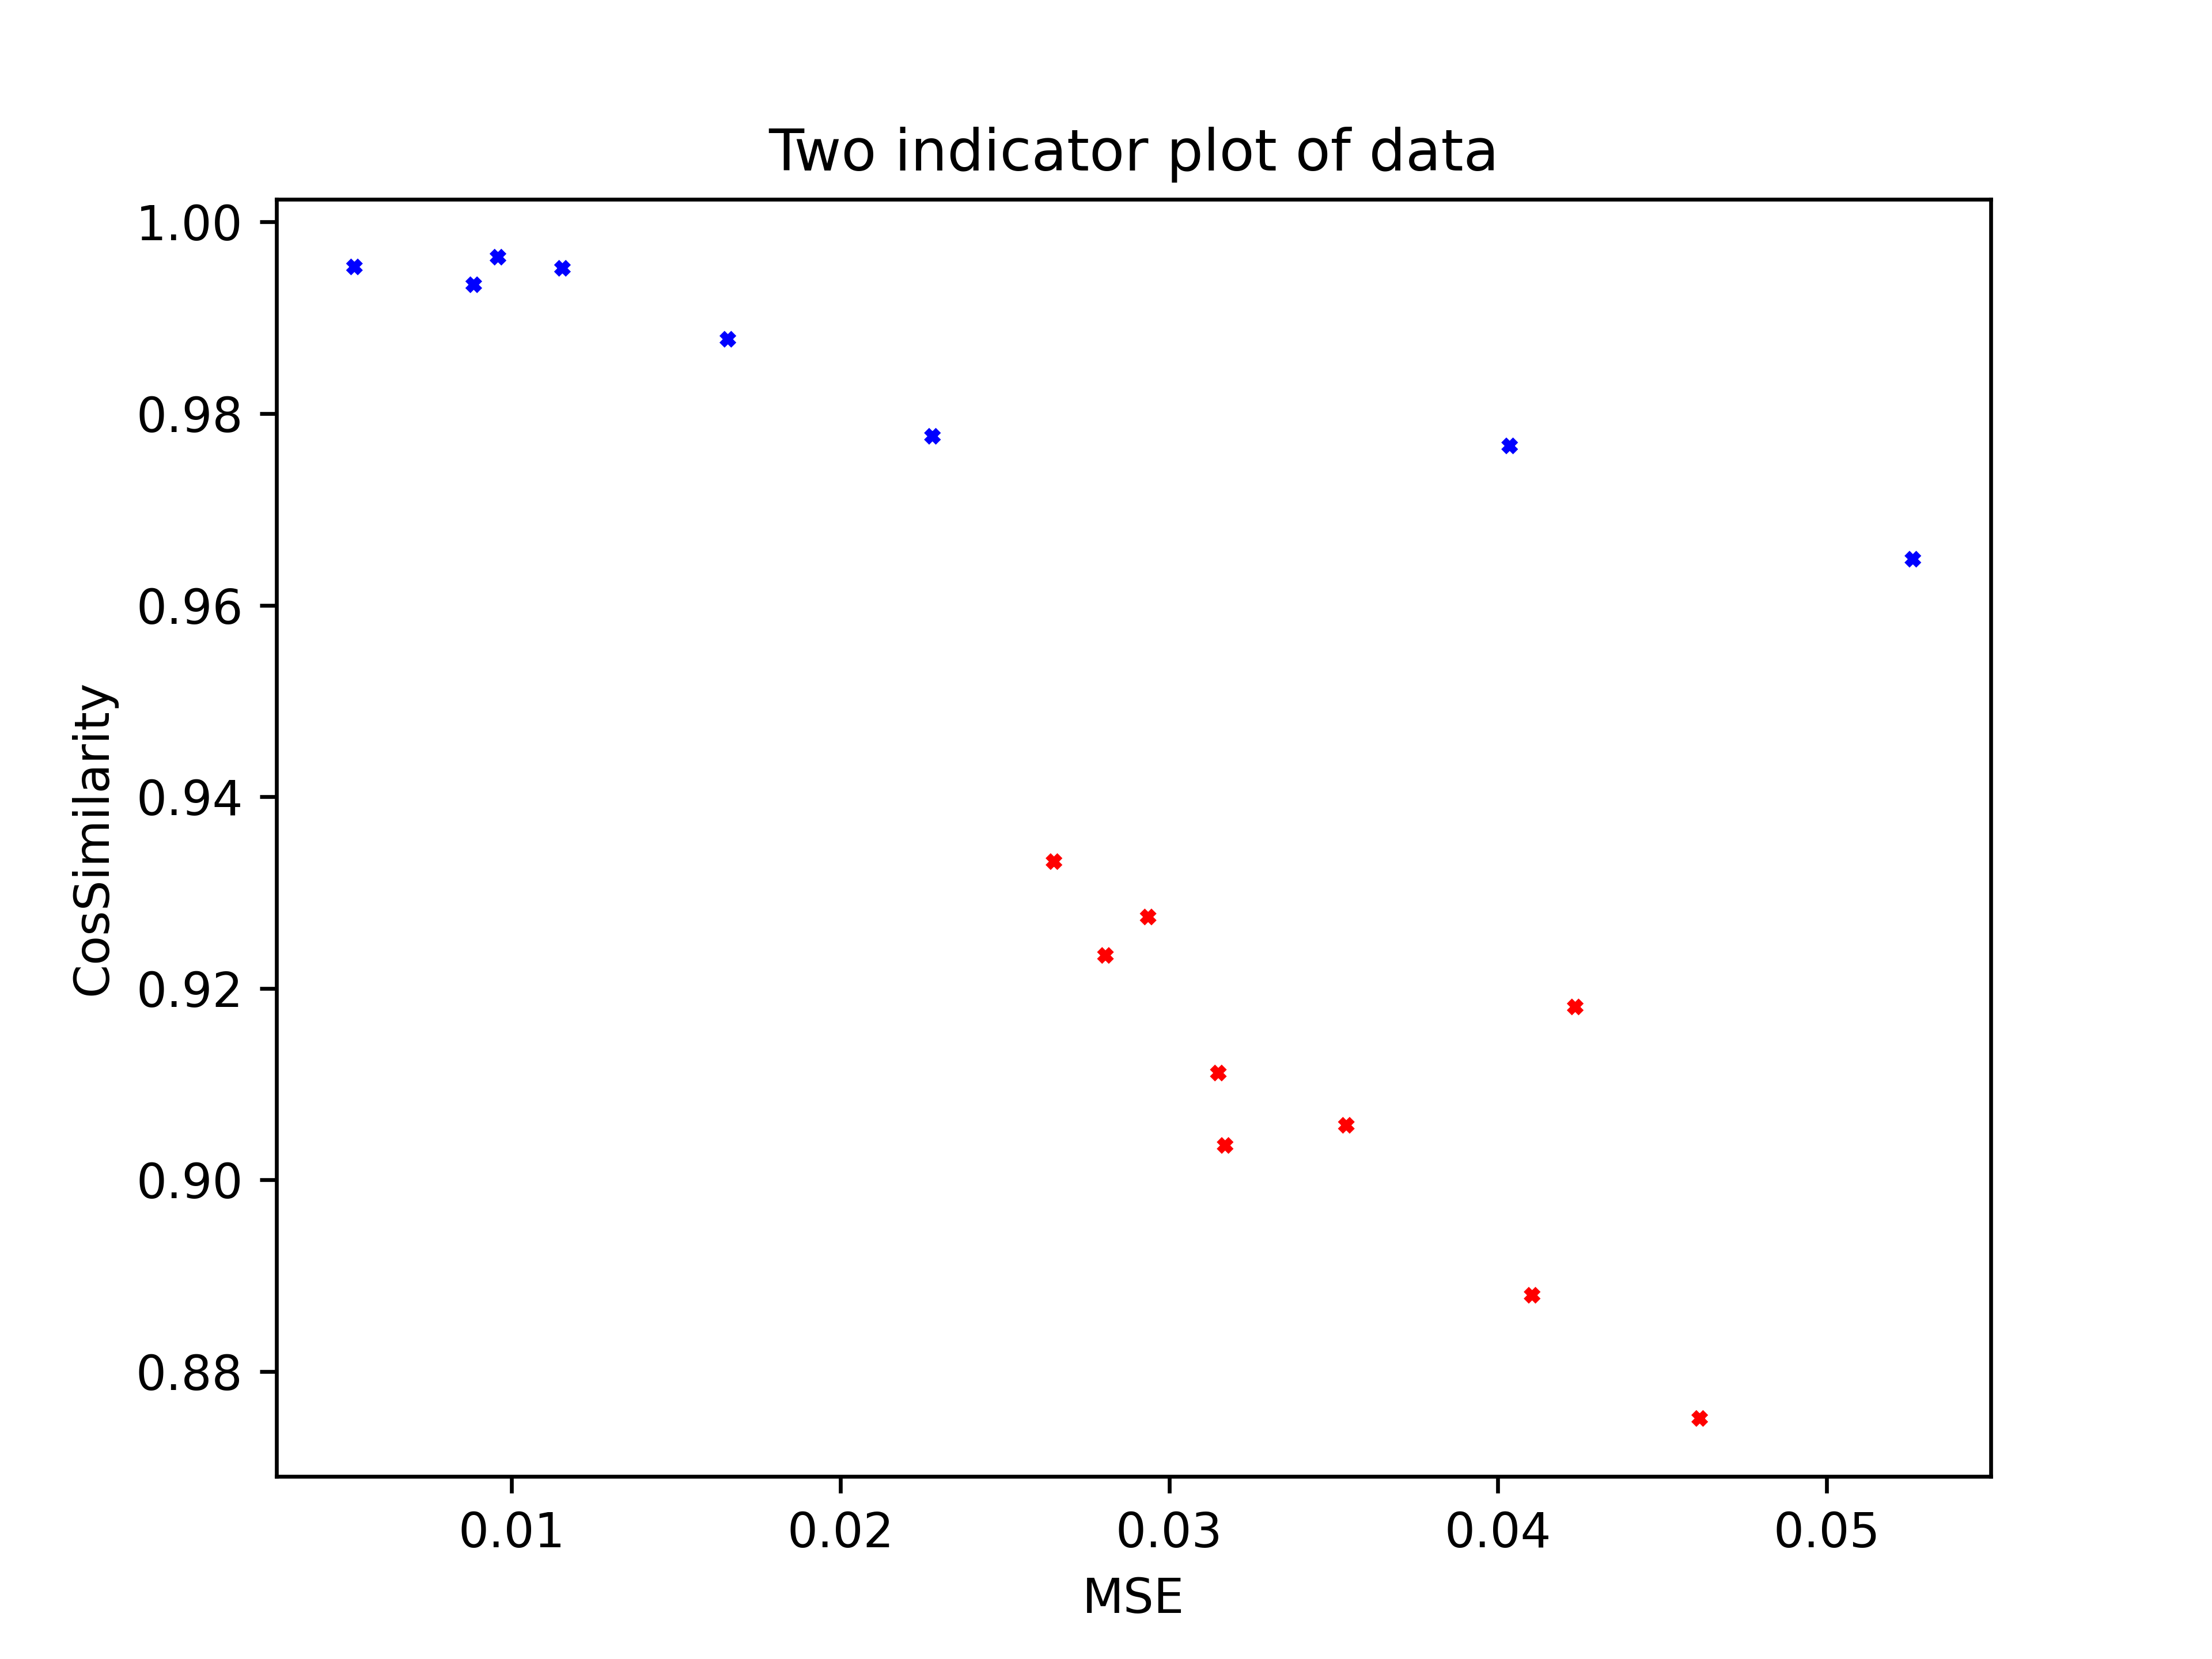
\includegraphics[width=4.0cm]{images/NewDoG_Streched_CSFed_A1_G_01r_23b_result.png}}
%  \vspace{1.5cm}
  \centerline{(c) DoG Model}\medskip
\end{minipage}
\hfill
\begin{minipage}[b]{0.48\linewidth}
  \centering
  \centerline{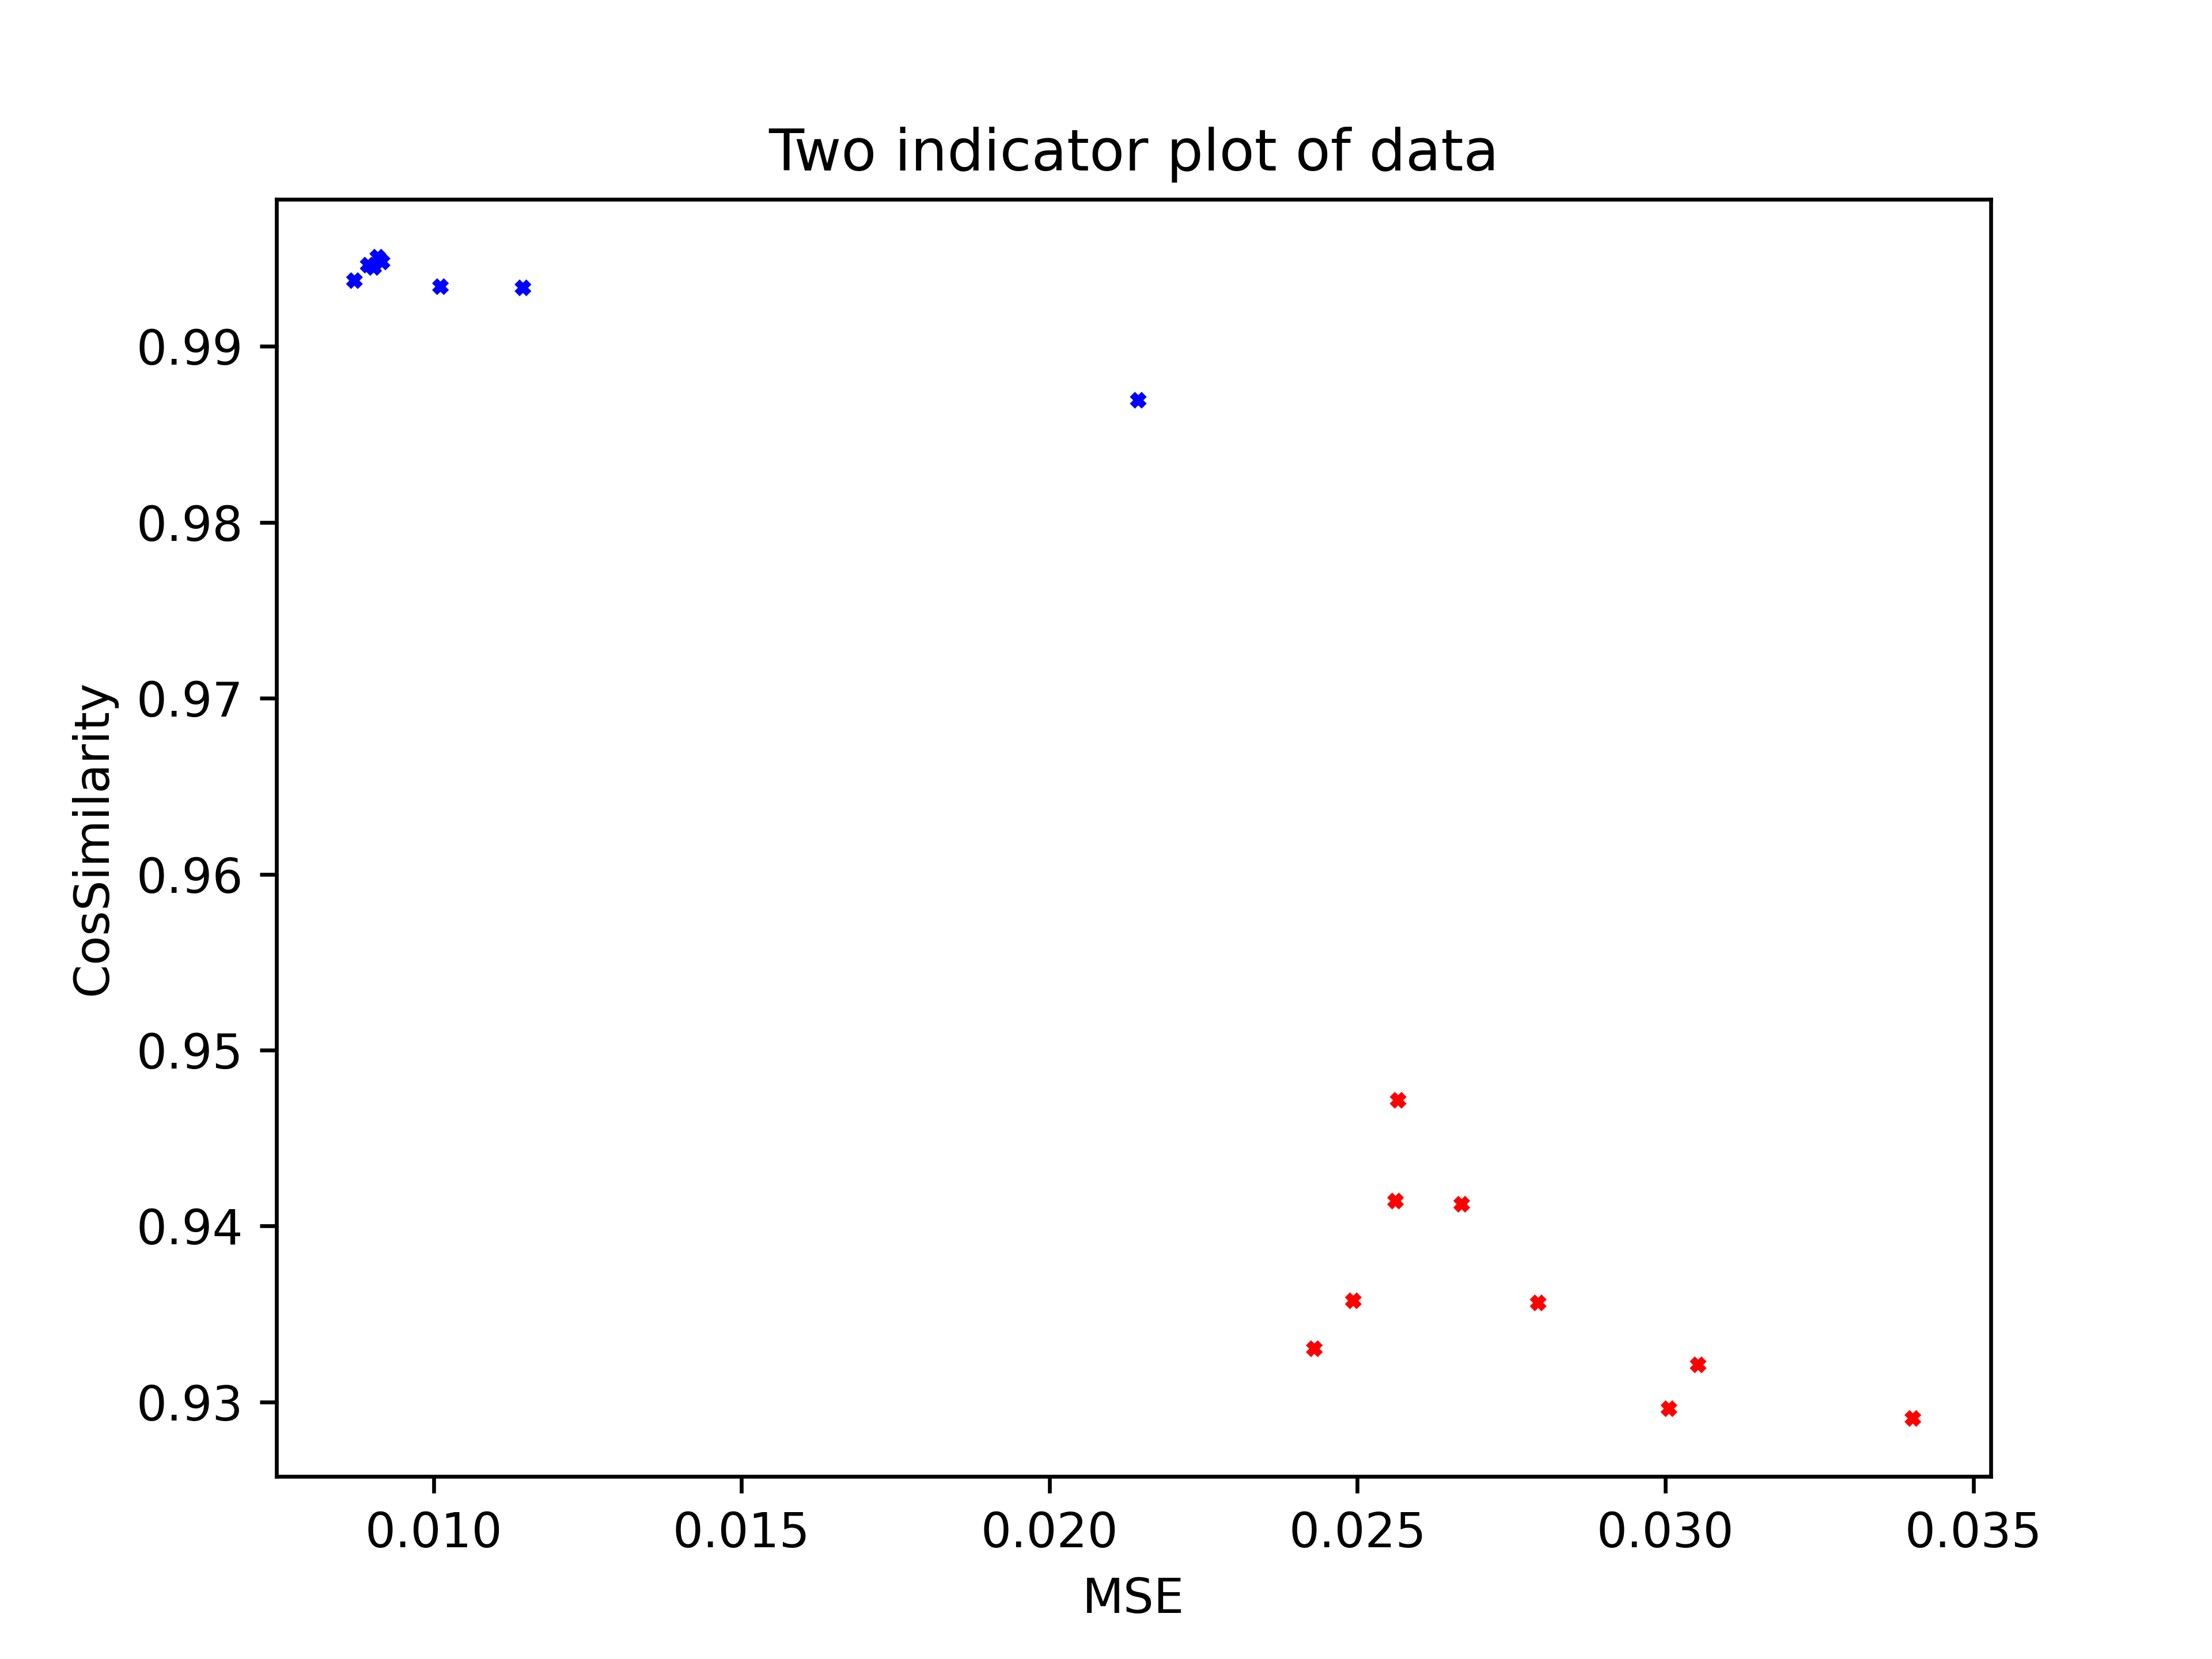
\includegraphics[width=4.0cm]{images/MS_STRECH_CSFED_G_A1_01r_23b_result.png}}
%  \vspace{1.5cm}
  \centerline{(d) Mannos and Sakrison Model}\medskip
\end{minipage}
\caption{Result of Different CSF Models}
\label{fig5}
%
\end{figure}
These plots that the Mannos and Sakrison model shows the clearest result which indicate the well compensated panel images and bad or not compensated panel images. 

\section{Conclusion and Future Work}
According to the experiment results, author concludes that the CSF - contrast sensitivity function, could play a fundamental role in a AMOLED display panel quality assessment system, it removes human visual system's subjective effect for judging quality of AMOLED display panel, it also improves the accuracy of the AMOLED display panel quality assessment system. By comparing the different CSF models, the results show that in this particular system, under same color and luminance condition, the Mannos and Sakriaon model of contrast sensitivity function has best overall performance. As the consideration of future work, Author is planning to train the system with larger image data-sets in order to find accurate good-bad quality decision boundary. This can lead to fine tune and build an automated AMOLED display panel quality assessment system.    

\clearpage
\begin{thebibliography}{8}
\bibitem{csf-humaneye} 
Peter G. J. Barten. 
"Contrast sensitivity of the human eye and its effects on image quality" ,
SPIE-The Intemational Society for Optical Engineering, 1999.

\bibitem{formulaOfCSF} 
Peter G.J. Barten.
"Formula for the contrast sensitivity of the human eye",
SPIE-The Intemational Society for Optical Engineering Vol.5294, 2004.

\bibitem{PhyModelOfCSF} 
Peter G.J. Barten.
"Physical Model For The Contrast Sensitivity of The Human Eye",
SPIE Vol. 1666 Human Vision, Visual Processing, and Digital Display III 1992.

\bibitem{Mannos-Sakrison}
James L. Mannos and Daivd J. Sakrison.
\textit{The Effects of a Visual Fidelity Criterion on the Encoding of Images}.
IEEE TRANSACTIONS ON INFORMATION THEORY, VOL. IT-20, No.4, 1974.

\bibitem{Ahumada}
A. J. Ahumada, Jr.
"Simplified Vision Models for Image Quality Assessment",
SID Digest pp. 397-400, NASA Ames Research Center, 1996.

\bibitem{Standard-Model-Contrast}
Andrew B. Watson and A. J. Ahumada, Jr.
"A Standard Model For Foveal Detection of Spatial Contrast",
Journal of Vision (2005)5, 717-740 , NASA Ames Research Center, 2005.

\bibitem{UseCSFinFusedIMage}
Zheng Liu and Wei Wu.
"The Use of the Contrast Sensitivity Function in the Perceptual Quality Assessment of Fused Image",
International Journal of Image and Data Fusion, Vol.2 No.1 P93-103, 2011

\bibitem{Movshon-Kiorpes}
J. Anthony Movshon and Lynne Kiorpes.
"Analysis of the development of spatial contrast sensitivity in monkey and human infants",
Journal Optical. Soc. Ameraca Vol.5, No.12, New York University, 1988

\bibitem{OnCS} 
Garrett M. Johnson and Mark D. Fairchild.
"On Contrast Sensitivity in an Image Difference Model", 
Rochester Institute of Technology.

\bibitem{AssessmentAlgoImageFusion}
Yin Chen, Rick S. Blum
"Methods for Measuring Display Defects and Mura as Correlated to Human Visual Perception",
ECE Department, Lehigh University, December 2007

\bibitem{657A_report}
Alyssa Huang and Tong Liu,"A CNN Based AMOLED Display Aging Compensation Quality Evaluation System", ECE Department, University of Waterloo, 2020

\bibitem{source}
Source code, "https://github.com/torontotong/UW-ECE613-Fall-2020-Research-Project.git".
\end{thebibliography}


\end{document}
